% Created 2017-02-19 Sun 15:58
% Intended LaTeX compiler: pdflatex
\documentclass[a4paper,11pt]{article}
\usepackage[utf8]{inputenc}
\usepackage[T1]{fontenc}
\usepackage{graphicx}
\usepackage{grffile}
\usepackage{longtable}
\usepackage{wrapfig}
\usepackage{rotating}
\usepackage[normalem]{ulem}
\usepackage{amsmath}
\usepackage{textcomp}
\usepackage{amssymb}
\usepackage{capt-of}
\usepackage{hyperref}
\usepackage[margin=1in]{geometry}
\usepackage{setspace}
\onehalfspacing
\usepackage{parskip}
\usepackage{amsthm}
\usepackage{amsmath}
\usepackage{mathtools}
\usepackage{hyperref}
\usepackage{graphicx}
\usepackage{tabularx}
\usepackage{booktabs}
\hypersetup{colorlinks,citecolor=black,filecolor=black,linkcolor=black,urlcolor=black}
\newtheorem{definition}{Definition}
\newtheorem{theorem}{Theorem}
\newcommand{\dx}{\mathrm{d}}
\newcommand{\var}{\mathrm{Var}}
\newcommand{\cov}{\mathrm{Cov}}
\newcommand{\corr}{\mathrm{Corr}}
\newcommand{\pr}{\mathrm{Pr}}
\newcommand{\rarrowd}[1]{\xrightarrow{\text{ \textit #1 }}}
\DeclareMathOperator*{\plim}{plim}
\newcommand{\plimn}{\plim_{n \rightarrow \infty}}
\setcounter{secnumdepth}{2}
\author{Zheng Tian}
\date{}
\title{Lecture 2: Review of Probability}
\hypersetup{
 pdfauthor={Zheng Tian},
 pdftitle={Lecture 2: Review of Probability},
 pdfkeywords={},
 pdfsubject={},
 pdfcreator={Emacs 25.1.1 (Org mode 9.0.3)}, 
 pdflang={English}}
\begin{document}

\maketitle
\setcounter{tocdepth}{1}
\tableofcontents

This lecture will review the basics in probability theory. The review
is by no means comprehensive. We will just refresh our mind with the
concepts that will be used the lectures that follow. 

\section{Random Variables and Probability Distributions}
\label{sec:orgcb9936c}

\subsection{Defining probabilities and random variables}
\label{sec:org54e1d8a}

\subsubsection*{Experiments, outcomes, sample space, and events}
\label{sec:org9a8be7d}

Probabilities are defined with respect to things whose occurrence are
random. We use the idea of an \textbf{experiment} to symbolize the processes
that generate random results. The \textbf{outcomes} of an experiment are its
mutually exclusive potential results. For example, a simple experiment
might be tossing a coin, the outcome of which is either getting a
head(H) or a tail(T) but not both.

We can denote all the outcomes from an experiment with a set \(S\), that
is called the \textbf{sample space}. In the tossing-coin experiment, the
sample space is \(\{H, T\}\). Or if we toss a dice, the sample space is
\(\{1, 2, 3, 4, 5, 6\}\). An \textbf{event} is a subset of the sample
space. Getting a head is an event, which is \(\{H\} \subset \{H, T\}\).

\subsubsection*{Probability}
\label{sec:org53fc231}

The \textbf{probability} of an event is the proportion of the time that the
event will occur in the long run. For example, we toss a coin for \(n\)
times and get \(m\) heads. When \(n\) is very large, we can say that the
probability of getting a head in a toss is \(m/n\). Obviously, we cannot
always repeat an experiment with infinite times. So we need a general
(axiomatic) definition of probability as follows.

\textbf{Definition of probability} A probability of an event \(A\)
in the sample space \(S\), denoted as \(\mathrm{Pr}(A)\), is a function
that assign \(A\) a real number in \([0, 1]\), satisfying the following
three conditions:
\begin{enumerate}
\item \(0 \leq \mathrm{Pr}(A) \leq 1\).
\item \(\mathrm{Pr}(S) = 1\).
\item For any disjoint sets, \(A\) and \(B\), that is \(A\) and \(B\) have no
element in common, \(\mathrm{Pr}(A \cup B) = \mathrm{Pr}(A) +
  \mathrm{Pr}(B)\).
\end{enumerate}

Here we use the concept of disjoint (or mutually exclusive) sets. \(A\)
and \(B\) are disjoint if there is no common element between these two
sets, that is, \(A \cap B\) is an empty set. 

\subsubsection*{Random variables}
\label{sec:org4b8d903}

Instead of using words or a set symbol to represent an event or an
outcome, we can use numeric value to do so. A \textbf{random variable} is
thus a numerical summary associated with the outcomes of an
experiment. You can also think of a random variable as a function
mapping from an event \(\omega\) in the sample space \(\Omega\) to the
real line, as illustrated in Figure \ref{fig:orgf661861}. 

\begin{figure}[htbp]
\centering
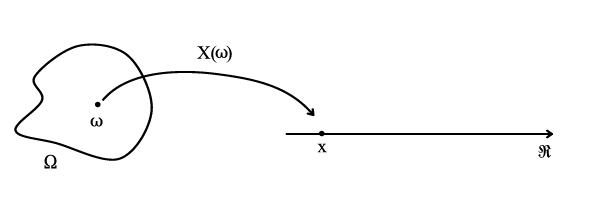
\includegraphics[width=0.8\textwidth]{figure/random_variable_demo1.png}
\caption{\label{fig:orgf661861}
An illustration of random variable}
\end{figure}

Random variables can take different types of values. A \textbf{discrete} random
variables takes on a discrete set of values, like \(0, 1, 2, \ldots, n\)
whereas a \textbf{continuous} random variable takes on a continuum of possble
values, like any value in the interval \((a, b)\). 


\subsection{Probability distributions}
\label{sec:org6e3a9bc}

\subsubsection*{The probability distribution for a discrete random variable}
\label{sec:org5da6f32}

The probability distribution of a discrete random variable is the list
of all possible values of the variable and the probability that each
value will occur. These probabilities sum to 1. 

\begin{itemize}
\item The probability mass function
\label{sec:org1c017c5}

Let \(X\) be a discrete random variable. The probability distribution of
\(X\) (or the probability mass function), \(p(x)\), is
\begin{equation*}
p(x) = \mathrm{Pr}(X = x)
\end{equation*}
where we use \(X\) to denote the random variable and \(x\) to denote a
specific value that \(X\) can take. We denote the set of all possible
value of \(X\) as \(S\). 

The axioms of probability require that (1) \(0 \leq p(x) \leq
1\) and (2) \(\sum_{ \{\text{all } x \text{ in } S \} } p(x) =
1\).

\begin{table}[htbp]
\caption{\label{tab:orgd6e1d7d}
An illustration of the probability distribution of a discrete random variable}
\centering
\begin{tabular}{lrrrr}
\toprule
\(X\) & 1 & 2 & 3 & Sum\\
\midrule
\(\mathrm{P}(x)\) & 0.25 & 0.75 & 0.25 & 1\\
\bottomrule
\end{tabular}
\end{table}

\item The cumulative probability distribution
\label{sec:org5c834c3}

The \textbf{cumulative probability distribution} (or the cumulative
distribution function, c.d.f.) is the probability that the random variable is
less than or equal to a particular value. Let \(F(x)\) be the c.d.f of
\(X\). Then \(F(x) = p(X \leq x)\). 

Table \ref{tab:org09e9954} and Figure \ref{fig:org907dba6} show that the
c.d.f. of a discrete random variable is a step function of \(x\). 

\begin{table}[htbp]
\caption{\label{tab:org09e9954}
An illustration of the c.d.f. of a discrete random variable}
\centering
\begin{tabular}{lrrrl}
\toprule
\(X\) & 1 & 2 & 3 & Sum\\
\midrule
\(\mathrm{P}(x)\) & 0.25 & 0.50 & 0.25 & 1\\
C.d.f. & 0.25 & 0.75 & 1 & --\\
\bottomrule
\end{tabular}
\end{table}

\begin{figure}[htbp]
\centering
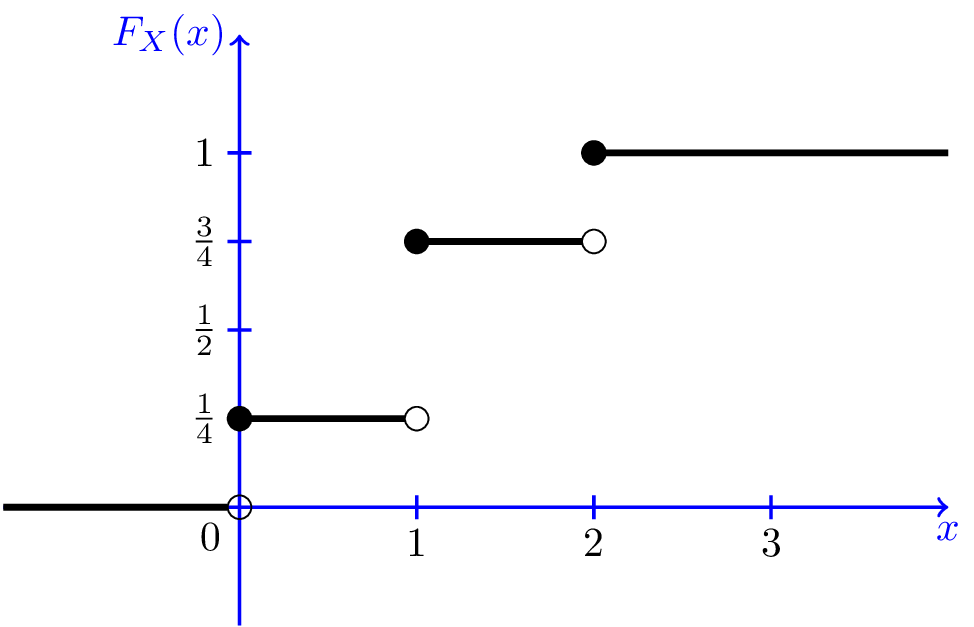
\includegraphics[width=0.53\textwidth,height=0.3\textheight]{figure/cdf_discrete_example.png}
\caption{\label{fig:org907dba6}
The c.d.f. of a discrete random variable}
\end{figure}

\item Bernouli distribution
\label{sec:org16ce5ba}

Many experiments like tossing a coin generate two outcomes: 1
with the probability of \(p\) and 0 with the probability of \(1-p\). The
random variable generated from such an experiment follows the Bernoulli
distribution. 

The Bernoulli distribution
\begin{equation*}
  G =
    \begin{cases}
      1 & \text{with probability } p \\
      0 & \text{with probability } 1-p
    \end{cases}
  \end{equation*}
\end{itemize}

\subsubsection*{The probability distribution of a continuous random variable}
\label{sec:org4644b80}

Unlike a discrete random variable that we can enumerate its values for
each corresponding event, a specific value of a continuous random
variable is just a point in the real line, the probability of which is
zero. Instead, we use the concept of the \textbf{probability density function
(p.d.f)} as the counterpart of the probability mass function. And the
definition of the p.d.f. of a continuous random variable depends on
the definition of its. c.d.f. 

The cumulative distribution function of a continous random variable
is defined as it is for a discrete random variable. That is, for a
continous random variable, \(X\), the c.d.f. is \(F(x) = \mathrm{Pr}(X
\leq x)\). And the \textbf{p.d.f.} of \(X\) is the function that satisfies 
\[ F(x) = \int_{-\infty}^{x} f(t) \mathrm{d}t \text{ for all } x \]

\begin{figure}[htbp]
\centering
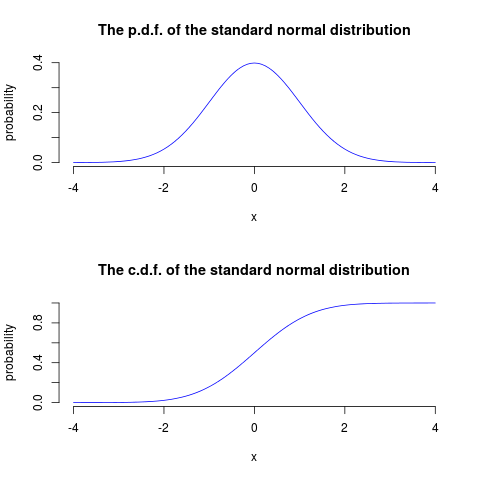
\includegraphics[width=0.6\textwidth,height=0.5\textheight]{figure/norm1.png}
\caption{\label{fig:org64af14d}
The p.d.f. and c.d.f. of a continuous random variable (the normal distribution)}
\end{figure}

For both discrete and continuous random variable, \(F(X)\) must satisfy
the following properties:
\begin{enumerate}
\item \(F(+\infty) = 1 \text{ and } F(-\infty) = 0\) (\(F(x)\) is bounded between 0 and 1)
\item \(x > y \Rightarrow F(x) \geq F(y)\) (\(F(x)\) is nondecreasing)
\end{enumerate}

By the definition of the c.d.f., we can conveniently calculate
probabilities, such as, 
\begin{itemize}
\item \(\mathrm{P}(x > a) = 1 - \mathrm{P}(x \leq a) = 1 - F(a)\)
\item \(\mathrm{P}(a < x \leq b) = F(b) - F(a)\).
\end{itemize}


\section{Expectation, Variance, and Other Moments}
\label{sec:org81d0055}

\subsection{The expected value of a random variable}
\label{sec:org5e41539}

\subsubsection*{Definition}
\label{sec:org9e3c167}

The \textbf{expected value} of a random variable, X, denoted as \(E(X)\), is
the long-run average of the random variable over many repeated
trials or occurrences, which is also called the \textbf{expectation} or the
\textbf{mean}. The expected value measures the centrality of a random
variable. 

\begin{itemize}
\item For a discrete random variable
\[ E(X) = \sum_{i=1}^n x_i \mathrm{Pr}(X = x_i) \]

e.g. The expectation of a Bernoulli random variable, G
  \[ E(G) = 1 \cdot p + 0 \cdot (1-p) = p \]

\item For a continuous random variable
\[ E(X) = \int_{-\infty}^{\infty} x f(x) \mathrm{d}x\]
\end{itemize}

\subsection{The variance and standard deviation}
\label{sec:orgebef600}

The \textbf{variance} of a random variable \(X\) measures its average
deviation from its own expected value. Let \(E(X) = \mu_X\) and denote
the variance of \(X\), denoted as \(\mathrm{Var}(X)\) or \(\sigma^2_X\), is then

\begin{equation*}
\mathrm{Var}(X) = E(X-\mu_X)^{2}=
\begin{cases}
\sum_{i=1}^n (x - \mu_X)^{2}\mathrm{Pr}(X = x_i) & \text{if } X \text{ is discrete} \\
\int_{-\infty}^{\infty} (x - \mu_X)^{2}f(x)\mathrm{d} x  & \text{if } X \text{ is continuous}
\end{cases}
\end{equation*}

The \textbf{standard deviation} of \(X\) is the square root of
\(\mathrm{Var}(X)\) and is denoted as \(\sigma_{X}\). That is,
\(\sigma_{X} = \sqrt{\mathrm{Var}(X)}\)

A convenient formula for calculating the variance is
\[ \mathrm{Var}(X) = E(X - \mu_X)^{2} = E(X^{2}) - \mu_X^{2} \]

The variance of a Bernoulli random variable, \(G\) 
\[ \mathrm{Var}(G) = (1-p)^{2}p + (0-p)^{2}(1-p) = p(1-p) \] and \(\sigma_{G} =
\sqrt{p(1-p)}\). 

From the definition of the expectation and variance, we can compute
the expectation and variance of a linear function of \(X\). Let \(Y = a +
bX\), then 
\begin{itemize}
\item \(E(Y) = a + E(X)\)
\item \(\mathrm{Var}(Y) = \mathrm{Var}(a + b X) = b^{2} \mathrm{Var}(X)\).
\end{itemize}


\subsection{Moments of a random variable, skewness and kurtosis}
\label{sec:org26b7320}

The expectation and variance are two special cases of the \textbf{moments} of
a distribution. 

\subsubsection*{Definition of the moments of a distribution}
\label{sec:org52c1323}

\begin{description}
\item[{k\(^{\text{th}}\) moment}] The k\(^{\text{th}}\) \textbf{moment} of the distribution of \(X\) is
\(E(X^{k})\). So, the expectation is the "first"
moment of \(X\).

\item[{k\(^{\text{th}}\) central moment}] The k\(^{\text{th}}\) central moment of the distribution
of \(X\) with its mean \(\mu_X\) is \(E(X - \mu_X)^{k}\). So, the
variance is the second central moment of \(X\).
\end{description}

It is important to remember that not all the moments of a distribution
exist. This is especially true for continuous random variables, for
which the integral to compute the moments may not converge. 

\subsubsection*{Skewness and kurtosis}
\label{sec:org14413fc}

We also use the third and fourth central moments to measure how a
distribution looks like asymmetric and how thick are its tails. 

\begin{itemize}
\item Skewness
\label{sec:orgd48f86f}

The skewness of a distribution provides a mathematical way to describe
how much a distribution deviates from symmetry. It is defined as 
\[ \text{Skewness} =  E(X - \mu_X)^{3}/\sigma_{X}^{3} \]

\begin{itemize}
\item A symmetric distribution has a skewness of zero.
\item The skewness can be either positive or negative.
\item That \(E(X - \mu_X)^3\) is divided by \(\sigma^3_X\) is to make the
skewness measure unit free. That is, changing the units of Y does
not change its skewness.
\end{itemize}

\item Kurtosis
\label{sec:orgb396f5f}

The kurtosis of the distribution of a random variable \(X\) measures how
much of the variance of \(X\) arises from extreme values, which makes
the distribution have "heavy" tails. 

The kurtosis of the distribution of \(X\) is 
\[ \text{Kurtosis} = E(X - \mu_X)^{4}/\sigma_{X}^{4} \]

\begin{itemize}
\item The kurtosis must be positive.
\item The kurtosis of the normal distribution is 3. So a distribution that
has its kurtosis exceeding 3 is called heavy-tailed, or
\textbf{leptokurtic}.
\item The kurtosis is also unit free.
\end{itemize}

Figure \ref{fig:org989b8bd} displays four distributions with different
skewness and kurtosis. All four distributions have a mean of zero and
a variance of one, while (a) and (b) are symmetric and (b)-(d) are
heavy-tailed. 

\begin{figure}[htbp]
\centering
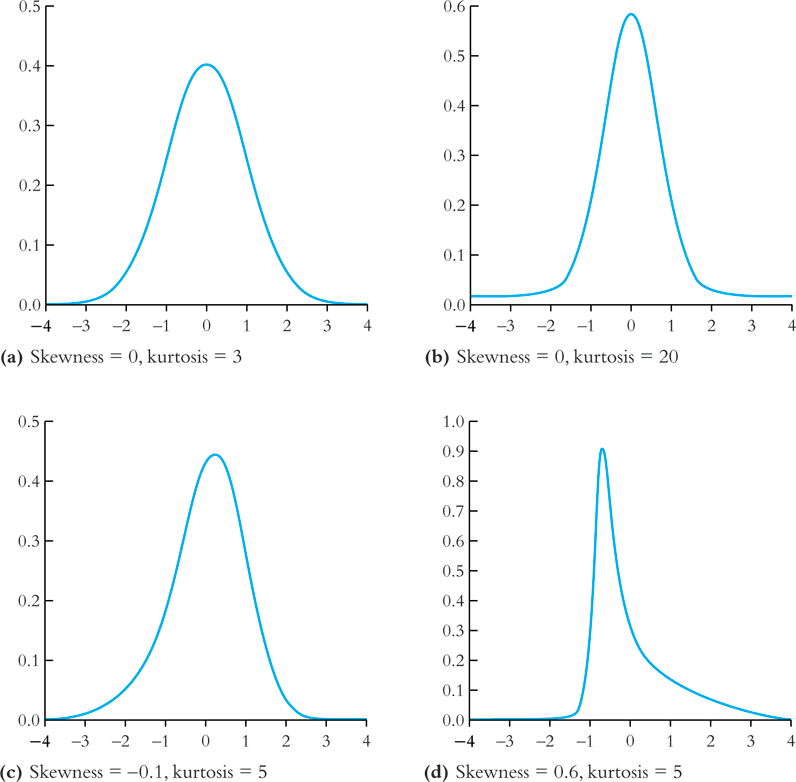
\includegraphics[width=0.6\textwidth]{figure/fig-2-3.png}
\caption{\label{fig:org989b8bd}
Four distributions with different skewness and kurtosis}
\end{figure}
\end{itemize}

\section{Two Random Variables}
\label{sec:org3723acc}
\subsection{The joint and marginal distributions}
\label{sec:org5f5c5b0}
\subsubsection*{The joint probability distributions}
\label{sec:org91ae5cb}
\begin{itemize}
\item The joint probability (density) functions
\label{sec:orgb1d5a65}

\begin{itemize}
\item For two discrete random variables \(X\) and \(Y\), the joint probability
distribution of \(X\) and \(Y\) is the probability that \(X\) and \(Y\)
simultaneously take on certain values, \(x\) and \(y\), that is
\[ p(x, y) = \mathrm{Pr}(X = x, Y = y)\]
which must satisfy the following
\begin{enumerate}
\item \(p(x, y) \geq 0\)
\item \(\sum_{x}\sum_{y} p(x, y) = 1\)
\end{enumerate}
\item For two continuous random variables, the counterpart of \(p(x, y)\) is
the joint probability density function, \(f(x, y)\), such that
\begin{enumerate}
\item \(f(x, y) \geq 0\)
\item \(\int_{x}\int_{y}f(x, y)\, \dx x\, \dx y= 1\)
\end{enumerate}
\end{itemize}
\end{itemize}

\subsubsection*{The marginal probability distribution}
\label{sec:org5a54bcd}
\begin{itemize}
\item The marginal probability (density) distribution
\label{sec:orga043683}

The marginal probability (density) distribution function of \(X\) is
computed from the joint probability (density) distribution function,
\(f(x, y)\) as
\begin{equation*}
f_{X}(x) =
\begin{cases}
\sum_{y} p(x, y) & \text{ in the discrete case} \\
\int_{y} f(x, y)\, \dx y & \text{ in the continuous case}
\end{cases}
\end{equation*}
\end{itemize}

\subsection{Conditional distributions}
\label{sec:org8333729}
\subsubsection*{The conditional probability}
\label{sec:org2732b80}
For any two events \(A\) and \(B\), the conditional probability of A given
B is defined as
\[ \mathrm{Pr}(A|B) = \frac{\mathrm{Pr}(A \cap B )}{\mathrm{Pr}(B)}\]
\subsubsection*{The conditional probability (density) distribution}
\label{sec:org4b26d92}
\begin{itemize}
\item For the discrete case, the conditional probability function is
\label{sec:org8f6e45d}

\[ p(x|y) = \frac{\mathrm{Pr}(X=x, Y=y)}{\mathrm{Pr}(Y=y)}\]

\item the continuous case, the conditional density function is
\label{sec:org6b5c5b5}
\[ f(x|y) = \frac{f(x, y)}{f_{Y}(y)}\]
\end{itemize}

\subsubsection*{The conditional expectation}
\label{sec:orgbef54f4}
\begin{itemize}
\item Definition
\label{sec:org9dcacd7}

\begin{equation*}
E(X|Y=y) =
\begin{cases}
\sum_{x}xp(x|y) & \text{ in the discrete case} \\
\int_{x}xf(x|y)\, \mathrm{d}x & \text{ in the continuous case}
\end{cases}
\end{equation*}

\item The law of iterated expectation: \(E(X) = E\left[E(X|Y)\right]\)
\label{sec:org146322c}

\begin{proof}
we prove the law of iterated expectation for the continuous case. The proof for the discrete case is similar.
\begin{align*}
E(X) & = \int_{x} xf_{X}(x)\, \mathrm{d}x \\
     & = \int_{x}\int_{y} xf(x, y)\, \mathrm{d}y\, \mathrm{d}x & \text{ by the definition of } f_{X}(x)) \\
     & = \int_{x}\int_{y} xf(x|y)f_{Y}(y)\, \mathrm{d}y\, \mathrm{dx} & \text{ by the definition of } f(x|y) \\
     & = \int_{y} \left[\int_{x} xf(x|y)\, \mathrm{d}x \right] f_{Y}(y)\, \mathrm{d}y & \text{ by the property of integral} \\
     & = \int_{y} E(X|Y=y)f_{Y}(y)\, \mathrm{d}y & \\
     & = E\left[E(X|Y)\right]
\end{align*}
\end{proof}

\begin{itemize}
\item If \(E(X|Y) = 0\), then \(E(X)=E\left[E(X|Y)\right]=0\).
\end{itemize}
\end{itemize}

\subsubsection*{Independence}
\label{sec:orgfd917ff}
Two random variables \(X\) and \(Y\) are \textbf{independent} if
\[ f(x|y) = f_{X}(x) \text{ or } f(y|x) = f_{Y}(y) \]

It follows that \(X\) and \(Y\) are independent if
\[ f(x, y) = f(x|y)f_{Y}(y) = f_{X}(x)f_{Y}(y) \]

\subsection{Covariance and Correlation}
\label{sec:org9f523d7}
\subsubsection*{Covariance}
\label{sec:org765c642}
The covariance of two random variables \(X\) and \(Y\) is
\[ \cov(X, Y) = E(X-\mu_{X})(Y-\mu_{Y}) \equiv \sigma_{XY} \]

The covariance can also be computed as
\[ \cov(X, Y) = E(XY) - E(X)E(Y) \]

If \(X\) and \(Y\) are independent, then
\begin{align*}
\cov(X, Y) & = \int_{x}\int_{y}(x - \mu_{x})(y - \mu_{Y})f(x, y)\, \dx(x)\, \dx(y) \\
& = \int_{x} (x - \mu_{X})f_{X}(x)\, \dx(x) \int_{y}(y - \mu_{Y})f_{Y}(y)\, \dx(y) \\
& = \left[E(X) - \mu_{X} \right] \left[ E(Y) - \mu_{Y} \right] \\
& = 0
\end{align*}

It means that if \(X\) and \(Y\) are independent, then they are
uncorrelated as well. But the opposite direction does not hold.

\subsubsection*{Correlation}
\label{sec:org3bcfb51}
The correlation coefficient between \(X\) and \(Y\) is given by
\[
\corr(X, Y) = \frac{\cov(X, Y)}{\left[\var(X)\var(Y)\right]^{1/2}} =
\frac{\sigma_{XY}}{\sigma_{X}\sigma_{Y}} \equiv \rho_{XY}
\]

\subsubsection*{Some useful operations}
\label{sec:org48b1892}
Let \(X\), \(Y\) be random variables, with the means \(\mu_{X}\) and
\(\mu_{Y}\), the variance \(\sigma^{2}_{X}\) and \(\sigma^{2}_{Y}\), and the
covariance \(\sigma_{XY}\), respectively. Then,
\begin{align*}
E(a + bX + cY) & = a + b \mu_{X} + c \mu_{Y} \\
\var(aX + bY)  & = a^{2} \sigma^{2}_{X} + b^{2} \sigma^{2}_{Y} + 2ab\sigma_{XY} \\
\cov(a + bX + cV, Y) & = b\sigma_{XY} + c\sigma_{VY} \\
\cov(X, Y) & \leq \sigma_{X}\sigma_{Y} \text{ and }  \corr(X, Y) \leq 1
\end{align*}


\section{Four Specific Distributions}
\label{sec:org1b1ccc8}
\subsection{The normal distribution}
\label{sec:org294d3eb}
\subsubsection*{Definition}
\label{sec:org36447e3}
The p.d.f. of a normally distributed random variable \(x\) is
\[ f(x) =
\frac{1}{\sigma\sqrt{2\pi}}\exp\left[-\frac{(x-\mu)^{2}}{2\sigma^{2}}\right]
\]
for which \(E(X) = \mu\) and \(\var(X) = \sigma^{2}\), and \(x\) is denoted
as \(x \sim N(\mu, \sigma^{2})\)

The standard normal distribution is a special case of the normal
distribution, for which \(\mu = 0\) and \(\sigma = 0\). The p.d.f of the
standard normal distribution is
\[
\phi(x) = \frac{1}{\sqrt{2\pi}}\exp\left(-\frac{x^2}{2}\right)
\]
The c.d.f of the standard normal distribution is often denoted as
\(\varPhi(x)\).

\subsubsection*{Transforming a normally distributed random variable to the standard normal distribution}
\label{sec:org8b25f8e}
Let \(X\) be a normally distributed random variable with the mean \(\mu\)
and the standard deviation \(\sigma\), i.e., \(X \sim N(\mu,
\sigma^2)\). Then \(Z = \frac{X - \mu}{\sigma}\) follows the standard
normal distribution, \(N(0, 1)\).

It follows that for any two number \(c_1 < c_2\) and let
\(d_1 = (c_1 - \mu)/\sigma\) and \(d_2 = (c_2 - \mu/\sigma)\), then
\begin{align*}
\mathrm{Pr}(X \leq c_2) & = \mathrm{Pr}(Z \leq d_2) = \varPhi(d_2) \\
\mathrm{Pr}(X \geq c_1) & = \mathrm{Pr}(Z \geq d_1) = 1 - \varPhi(d_1) \\
\mathrm{Pr}(c_1 \leq X \leq c_2) & = \mathrm{Pr}(d_1 \leq Z \leq d_2) = \varPhi(d_2) - \varPhi(d_1)
\end{align*}

\begin{center}
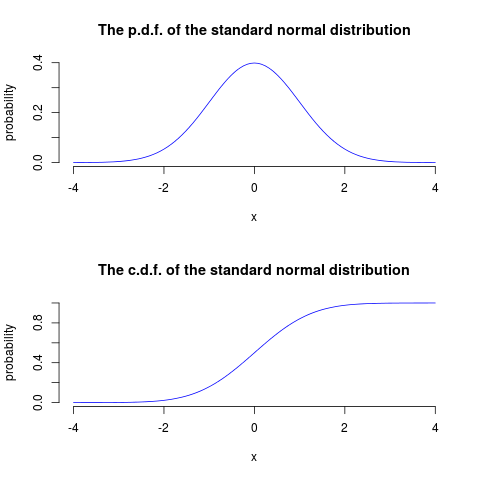
\includegraphics[width=.9\linewidth]{figure/norm1.png}
\end{center}

\subsubsection*{The multivariate normal distribution}
\label{sec:orga62a12b}
The normal distribution can be generalized to describe the joint
distribution of a set of random variables, which have the multivariate
normal distribution. (See Appendix 17.1 for the p.d.f of this
distribution and the special case of the bivariate normal
distribution.)

\begin{itemize}
\item Important properties of the multivariate normal distribution
\label{sec:orgdb2c586}

\begin{enumerate}
\item If \(X\) and \(Y\) have a bivariate normal distribution with covariance
\(\sigma_{XY}\) and \(a\) and \(b\) are two constants, then
\[
   aX + bY \sim N(a\mu_X + b\mu_Y, a^2\sigma_X + b^2\sigma_Y +
   2ab\sigma_{XY})
   \]

More generally, if n random variables, \(x_1, \ldots, x_n\), have a
multivariate normal distribution, then any linear combination of
these variables is normally distributed, for example, \(\sum_{i=1}^n
   x_i\). For any real numbers, \(\alpha_1, \ldots, \alpha_n\), a linear
combination of \({x_i}\) is \(\sum_i \alpha_i x_i\).

\item If a set of random variables has a multivariate normal
distribution, then the marginal distribution of each of the
variables is normal.

\item If random variables with a multivariate normal distribution have
covariances that equal zero, then these random variables are
independent.

Let \(X\) and \(Y\) be two random variables with a bivariate normal
distribution. The joint p.d.f of \(X\) and \(Y\) is \(f(x, y)\), with the
marginal p.d.f. being \(f_X(x)\) and \(f_Y(y)\), respectively. Then we have
\[ \cov(X, Y) = 0 \Leftrightarrow f(x, y) = f_X(x)f_Y(y) \]

\textbf{Note}: this property only holds for random variables with a
multivariate normal distribution. Generally, uncorrelation does not
imply independence.

\item If \(X\) and \(Y\) have a bivariate normal distribution, then
\[E(Y|X = x) = a + bx \]
where \(a\) and \(b\) are constants.
\end{enumerate}
\end{itemize}

\subsection{The chi-squared distribution}
\label{sec:orge7ec5ce}
Let \(Z_1, \ldots, Z_n\) be n indepenent standard normal distribution,
i.e. \(Z_i \sim N(0, 1)\) for all \(i = 1, \ldots, n\). The random
variable
\[W = \sum_{i=1}^n Z^2_i \]
has a chi-squared distribution with \(n\) degrees of freedom, denoted as
\(W \sim \chi^2(n)\), with \(E(W) = n\) and \(\var(W) = 2n\)

e.g. If \(Z \sim N(0, 1)\), then \(W = Z^2 \sim \chi^2(1)\) with \(E(W) =
1\) and \(\var(W) = 2\).

\subsection{The student t distribution}
\label{sec:org946965d}
Let \(Z \sim N(0, 1)\), \(W \sim \chi^2(m)\), and let \(Z\) and \(W\) be
independently distributed. Then the random variable
\[t = \frac{Z}{\sqrt{W/m}} \]
has a student t distribution with \(m\) degrees of freedom, denoted as
\(t \sim t(m)\).

As \(n \rightarrow \infty\), \(t\) has a standard normal distribution.

\subsection{The F distribution}
\label{sec:orgebf0ed3}
Let \(W_1 \sim \chi^2(n_1)\), \(W_2 \sim \chi^2(n_2)\), and \(W_1\) and
\(W_2\) are independent. Then the random variable
\[ F = \frac{W_1/n_1}{W_2/n_2}\]
has an F distribution with \((n_1, n_2)\) degrees of freedom, denoted as
\(F \sim F(n_1, n_2)\)

\begin{itemize}
\item If \(t \sim t(n)\), then \(t^2 \sim F(1, n)\)
\item As \(n_2 \rightarrow \infty\), the \(F(n_1, \infty)\) distribution is the
same as the \(\chi^2(n_1)\) distribution, divided by \(n_1\).
\end{itemize}


\section{Random Sampling and the Distribution of the Sample Average}
\label{sec:org2aa0f54}
\subsection{Random sampling}
\label{sec:orgfd9198a}
\begin{description}
\item[{Simple random sampling}] \(n\) objects are selected at random from a
\textbf{population}, and each member of the population is equally likely
to be included in the sample

\item[{i.i.d. draws}] when \(Y_1, Y_2, \ldots, Y_n\) are drawn from the same
distribution and are independently distributed, they
are said to be \textbf{independently and identically
distributed} or \textbf{i.i.d}. This fact can be denoted as
\(Y_i \sim IID(\mu_Y, \sigma^2_Y)\) for \(i = 1, 2,
                  \ldots, n\).
\end{description}

\subsection{The sampling distribution of the sample average}
\label{sec:org2276567}
\subsubsection*{The sample average}
\label{sec:org96653ed}
The \textbf{sample average} or \textbf{sample mean}, \(\overline{Y}\), of the \(n\)
observation \(Y_1, Y_2, \ldots, Y_n\) is
\[ \overline{Y} = \frac{1}{n}\sum^n_{i=1} Y_i \]
Note that since \(Y_i\) is random, so is \(\overline{Y}\).

\subsubsection*{The mean and variance of \(\overline{Y}\)}
\label{sec:orga6af3ab}
Suppose that \(Y_i \sim IID(\mu_Y, \sigma^2_{Y})\) for all \(i = 1,
\ldots, n\). Then, by the definition of \(\overline{Y}\) and the fact
that \(Y_i\) and \(Y_j\) are independent for any \(i \neq j\), implying
\(\cov(Y_i, Y_j)=0\), we have
\[
E(\overline{Y}) =
\frac{1}{n}\sum^n_{i=1}E(Y_i) = \frac{1}{n}\cdot n\mu_Y = \mu_Y
\]
and
\[
\var(\overline{Y}) = \frac{1}{n^2}\sum^n_{i=1}\var(Y_i) +
\frac{1}{n^2}\sum^n_{i=1}\sum^n_{j=1}\cov(Y_i, Y_j) =
\frac{\sigma^2_Y}{n}
\]

e.g. If \(Y_1, \ldots, Y_n\) are i.i.d. draws from \(N(\mu_Y,
\sigma^2_Y)\), then \(\overline{Y} \sim N(\mu_Y, \sigma^2_Y/n)\).


\section{Large Sample Approximations to Sampling Distributions}
\label{sec:org3d61c89}
\subsection{The law of large numbers}
\label{sec:org3c9523d}
\subsubsection*{Convergence in probability}
\label{sec:org9a57a15}
Let \(S_1, \ldots, S_n, \ldots\) be a sequence of random variables,
denoted as \(\{S_n\}\). \(\{S_n\}\) is said to converge in probability to a
limit \(\mu\) that is, \(S_n \xrightarrow{\text{ \textit p }} \mu\), if and only if
\[ \mathrm{Pr} \left(|S_n-\mu| \geq \delta \right) \rightarrow 0 \]
as \(n \rightarrow \infty\) for every \(\delta > 0\).

\begin{itemize}
\item e.g. \(S_n = \overline{Y}\). That is, \(S_1=Y_1\), \(S_2=1/2(Y_1+Y_2)\),
\(S_n=1/n\sum_i Y_i\), and so forth.
\end{itemize}

\subsubsection*{The law of large numbers}
\label{sec:org7f66606}
If \(Y_1, \ldots, Y_n\) are i.i.d., \(E(Y_i)=\mu_Y\) and \(\var(Y_i) <
\infty\), then \(\overline{Y} \xrightarrow{\text{ \textit p }} \mu_Y\)

\begin{figure}[htbp]
\centering
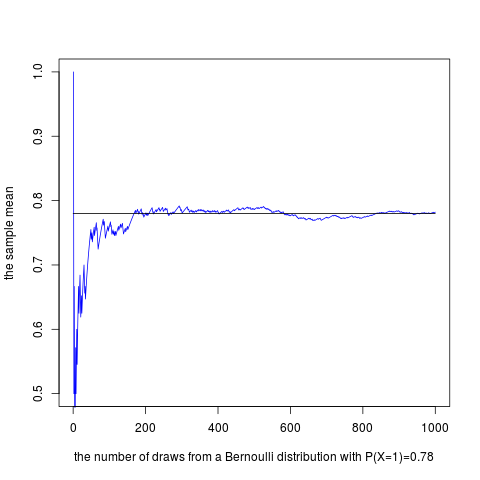
\includegraphics[width=0.75\textwidth]{figure/demo_lln.png}
\caption{An illustration of the law of large numbers}
\end{figure}

\subsection{The central limit theorem}
\label{sec:org9e9f985}
\subsubsection*{Convergence in distribution}
\label{sec:org09b3935}
Let \(F_1, F_2, \ldots, F_n, \ldots\) be a sequence of cumulative
distribution functions corresponding to a sequence of random
variables, \(S_1, S_2, \ldots, S_n, \ldots\). Then the sequence of
random variables \(S_n\) is said to \textbf{converge in distribution} to \(S\),
denoted as \(S_n \xrightarrow{\text{ \textit d }} S\), if the
distribution functions \(\{F_n\}\) converge to \(F\), the distribution
function of \(S\). That is,
\[ S_n \xrightarrow{\text{ \textit d }} S \text{ if and only if } \lim_{n
\rightarrow \infty}F_n(t)=F(t) \]
where the limit holds at all points \(t\) at which the limiting
distribution \(F\) is continuous. The distribution \(F\) is called the
\textbf{asymptotic distribution} of \(S_n\).

\subsubsection*{The central limit theorem (Lindeberg-Levy CLT)}
\label{sec:orgb84cffb}
If \(Y_1, Y_2, \ldots, Y_n\) are i.i.d. random samples from a
probability distribution with finite mean \(\mu_Y\) and finite variance
\(\sigma^2_Y\), i.e., \(0 < \sigma^2_Y < \infty\) and \(\overline{Y} =
(1/n)\sum_i^nY_i\). Then
\[ \sqrt{n}(\overline{Y}-\mu_Y) \xrightarrow{\text{ \textit d }} N(0,
\sigma^2_Y) \]
It follows that since \(\sigma_{\overline{Y}} =
\sqrt{\var(\overline{Y})} = \sigma_Y/\sqrt{n}\),
\[ \frac{\overline{Y} - \mu_Y}{\sigma_{\overline{Y}}}
\xrightarrow{\text{ \textit d }} N(0, 1) \]

\begin{figure}[htbp]
\centering
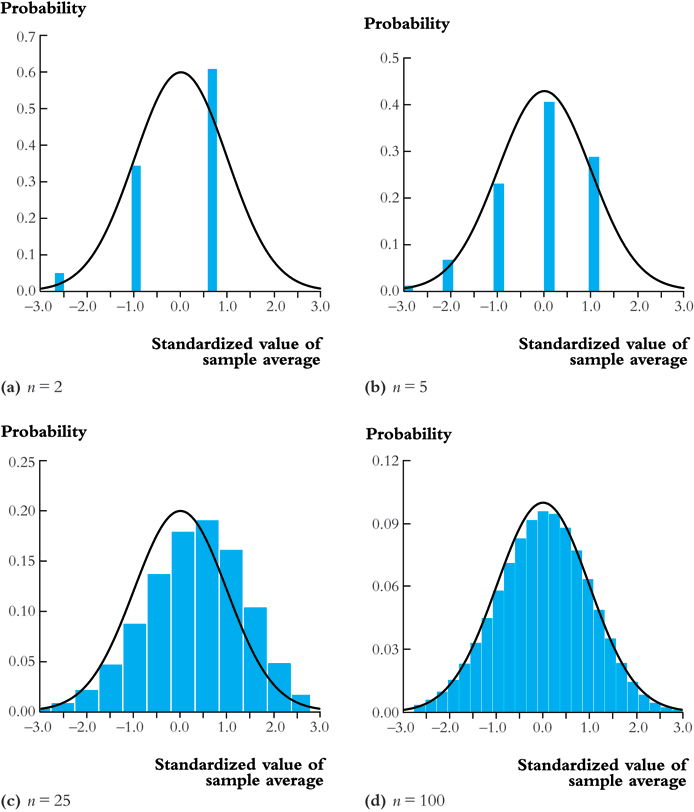
\includegraphics[width=0.8\textwidth]{figure/fig-2-9.png}
\caption{Distribution of the standardized sample average of n Bernoulli random variable with p = 0.78}
\end{figure}
\end{document}